\hypertarget{the-theory-of-evolution-1}{%
\chapter{The Theory of Evolution}\label{the-theory-of-evolution-1}}

\href{https://en.wikipedia.org/wiki/Evolution}{Evolution} is change in the heritable characteristics of biological populations over successive generations. These characteristics are the expressions of genes that are passed on from parent to offspring during reproduction. Different characteristics tend to exist within any given population as a result of mutation, genetic recombination and other sources of genetic variation. Evolution occurs when evolutionary processes such as natural selection (including sexual selection) and genetic drift act on this variation, resulting in certain characteristics becoming more common or rare within a population. It is this process of evolution that has given rise to biodiversity at every level of biological organisation, including the levels of species, individual organisms and molecules.

Repeated formation of new species (speciation), change within species (anagenesis), and loss of species (extinction) throughout the evolutionary history of life on Earth are demonstrated by shared sets of morphological and biochemical traits, including shared DNA sequences. These shared traits are more similar among species that share a more recent common ancestor, and can be used to reconstruct a biological ``tree of life'' based on evolutionary relationships (phylogenetics), using both existing species and fossils. The fossil record includes a progression from early biogenic graphite, to microbial mat fossils, to fossilized multicellular organisms. Existing patterns of biodiversity have been shaped both by speciation and by extinction.

\href{https://en.wikipedia.org/wiki/Charles_Darwin}{Charles Darwin} developed his theory of ``natural selection'' from 1838 onwards and was writing up his ``big book'' on the subject when \href{https://en.wikipedia.org/wiki/Alfred_Russel_Wallace}{Alfred Russel Wallace} sent him a version of virtually the same theory in 1858. Their separate papers were presented together at an 1858 meeting of the Linnaean Society of London. At the end of 1859, Darwin's book ``On the Origin of Species'' explained natural selection in detail and in a way, that led to an increasingly wide acceptance of Darwin's concepts of evolution at the expense of alternative theories.

According to \href{https://en.wikipedia.org/wiki/Ernst_Mayr}{Ernst Mayr}, Darwin's theory actually consists of a number of different theories that can be best understood when they are clearly distinguished from each other. Mayr distinguished five independent theories:

\begin{enumerate}
\def\labelenumi{\arabic{enumi}.}
\tightlist
\item
  The non-constancy of species (the basic theory of evolution)
\item
  The descent of all organisms from common ancestors (branching evolution)
\item
  The gradualness of evolution (no saltations, no discontinuities)
\item
  The multiplication of species (the origin of diversity)
\item
  Natural selection
\end{enumerate}

The first and second theories were widely accepted by biologists rather quickly following Darwin's publication. The other three theories were not widely accepted until the arrival of the so-called modern synthesis in the 20th century (see below).

Evolution by \href{https://en.wikipedia.org/wiki/Natural_selection}{natural selection} is a process demonstrated by the observation that more offspring are produced than can possibly survive, along with three facts about populations: 1) traits vary among individuals with respect to morphology, physiology, and behavior (phenotypic variation), 2) different traits confer different rates of survival and reproduction (differential fitness), and 3) traits can be passed from generation to generation (heritability of fitness). Thus, in successive generations members of a population are replaced by progeny of parents better adapted to survive and reproduce in the biophysical environment in which natural selection takes place.

The four most widely recognized evolutionary processes are natural selection (including sexual selection), \href{https://en.wikipedia.org/wiki/Genetic_drift}{genetic drift}, \href{https://en.wikipedia.org/wiki/Mutation}{mutation} and \href{https://en.wikipedia.org/wiki/Gene_flow}{gene migration} due to genetic admixture. Natural selection and genetic drift sort variation; mutation and gene migration create variation.

The mechanisms of reproductive heritability and the origin of new traits remained a mystery. Towards this end, Darwin developed his provisional theory of pangenesis. In 1865, \href{https://en.wikipedia.org/wiki/Gregor_Mendel}{Gregor Mendel} reported that traits were inherited in a predictable manner through the independent assortment and segregation of elements (later known as genes). Mendel's laws of inheritance eventually supplanted most of Darwin's pangenesis theory. \href{https://en.wikipedia.org/wiki/August_Weismann}{August Weismann} made the important distinction between germ cells that give rise to gametes (such as sperm and egg cells) and the somatic cells of the body, demonstrating that heredity passes through the germ line only. \href{https://en.wikipedia.org/wiki/Hugo_de_Vries}{Hugo de Vries} connected Darwin's pangenesis theory to Weismann's germ/soma cell distinction and proposed that Darwin's pangenes were concentrated in the cell nucleus and when expressed they could move into the cytoplasm to change the cells structure. de Vries was also one of the researchers who made Mendel's work well-known, believing that Mendelian traits corresponded to the transfer of heritable variations along the germline. de Vries developed a mutation theory to explain how new variants originate. This led to a temporary rift between those who accepted Darwinian evolution and biometricians who allied with de Vries. In the 1930s, pioneers in the field of population genetics, such as \href{https://en.wikipedia.org/wiki/Ronald_Fisher}{Ronald Fisher}, \href{https://en.wikipedia.org/wiki/Sewall_Wright}{Sewall Wright} and \href{https://en.wikipedia.org/wiki/J._B._S._Haldane}{J. B. S. Haldane} set the foundations of evolution onto a robust statistical philosophy. The false contradiction between Darwin's theory, genetic mutations, and Mendelian inheritance was thus reconciled.

In the 1920s and 1930s the so-called \href{https://en.wikipedia.org/wiki/Modern_synthesis_(20th_century)}{modern synthesis} connected natural selection and population genetics, based on Mendelian inheritance, into a unified theory that applied generally to any branch of biology. The modern synthesis explained patterns observed across species in populations, through fossil transitions in paleontology, and complex cellular mechanisms in developmental biology. The publication of the structure of \href{https://en.wikipedia.org/wiki/DNA}{DNA} by \href{https://en.wikipedia.org/wiki/James_Watson}{James Watson} and \href{https://en.wikipedia.org/wiki/Francis_Crick}{Francis Crick} in 1953 demonstrated a physical mechanism for inheritance. Molecular biology improved our understanding of the relationship between genotype and phenotype. Advancements were also made in phylogenetic systematics, mapping the transition of traits into a comparative and testable framework through the publication and use of evolutionary trees. In 1973, evolutionary biologist \href{https://en.wikipedia.org/wiki/Theodosius_Dobzhansky}{Theodosius Dobzhansky} penned that ``nothing in biology makes sense except in the light of evolution,'' because it has brought to light the relations of what first seemed disjointed facts in natural history into a coherent explanatory body of knowledge that describes and predicts many observable facts about life on this planet.

All life on Earth shares a common ancestor known as the \href{https://en.wikipedia.org/wiki/Last_universal_common_ancestor}{last universal common ancestor} (LUCA), which lived approximately 3.5--3.8 billion years ago. The fossil record includes a progression from early biogenic graphite, to microbial mat fossils, to fossilised multicellular organisms. Existing patterns of biodiversity have been shaped by repeated formations of new species (speciation), changes within species (anagenesis) and loss of species (extinction) throughout the evolutionary history of life on Earth. Morphological and biochemical traits are more similar among species that share a more recent common ancestor, and can be used to reconstruct phylogenetic trees.

In terms of practical application, an understanding of evolution has been instrumental to developments in numerous scientific and industrial fields, including agriculture, human and veterinary medicine, and the life sciences in general. Discoveries in evolutionary biology have made a significant impact not just in the traditional branches of biology but also in other academic disciplines, including biological anthropology, and evolutionary psychology.

\hypertarget{history-of-evolutionary-thought}{%
\section{History of Evolutionary Thought}\label{history-of-evolutionary-thought}}

The proposal that one type of organism could descend from another type goes back to some of the first pre-Socratic Greek philosophers, such as Anaximander and Empedocles. Such proposals survived into Roman times.

In contrast to these materialistic views, Aristotelianism considered all natural things as actualisations of fixed natural possibilities, known as forms. This was part of a medieval teleological understanding of nature in which all things have an intended role to play in a divine cosmic order. Variations of this idea became the standard understanding of the Middle Ages and were integrated into Christian learning, but Aristotle did not demand that real types of organisms always correspond one-for-one with exact metaphysical forms and specifically gave examples of how new types of living things could come to be.

In the 17th century, the new method of modern science rejected the Aristotelian approach. It sought explanations of natural phenomena in terms of physical laws that were the same for all visible things and that did not require the existence of any fixed natural categories or divine cosmic order. However, this new approach was slow to take root in the biological sciences, the last bastion of the concept of fixed natural types. John Ray applied one of the previously more general terms for fixed natural types, ``species'', to plant and animal types, but he strictly identified each type of living thing as a species and proposed that each species could be defined by the features that perpetuated themselves generation after generation. The biological classification introduced by Carl Linnaeus in 1735 explicitly recognised the hierarchical nature of species relationships, but still viewed species as fixed according to a divine plan.

Other naturalists of this time speculated on the evolutionary change of species over time according to natural laws. In 1751, Pierre Louis Maupertuis wrote of natural modifications occurring during reproduction and accumulating over many generations to produce new species. Georges-Louis Leclerc, Comte de Buffon suggested that species could degenerate into different organisms, and Erasmus Darwin proposed that all warm-blooded animals could have descended from a single microorganism (or ``filament''). The first full-fledged evolutionary scheme was Jean-Baptiste Lamarck's ``transmutation'' theory of 1809, which envisaged spontaneous generation continually producing simple forms of life that developed greater complexity in parallel lineages with an inherent progressive tendency, and postulated that on a local level, these lineages adapted to the environment by inheriting changes caused by their use or disuse in parents. (The latter process was later called Lamarckism.) These ideas were condemned by established naturalists as speculation lacking empirical support. In particular, Georges Cuvier insisted that species were unrelated and fixed, their similarities reflecting divine design for functional needs. In the meantime, Ray's ideas of benevolent design had been developed by William Paley into the Natural Theology or Evidences of the Existence and Attributes of the Deity (1802), which proposed complex adaptations as evidence of divine design and which was admired by Charles Darwin.

The crucial break from the concept of constant typological classes or types in biology came with the theory of evolution through natural selection, which was formulated by Charles Darwin in terms of variable populations. Darwin used the expression ``descent with modification'' rather than ``evolution''. Partly influenced by An Essay on the Principle of Population (1798) by Thomas Robert Malthus, Darwin noted that population growth would lead to a ``struggle for existence'' in which favourable variations prevailed as others perished. In each generation, many offspring fail to survive to an age of reproduction because of limited resources. This could explain the diversity of plants and animals from a common ancestry through the working of natural laws in the same way for all types of organism. Darwin developed his theory of ``natural selection'' from 1838 onwards and was writing up his ``big book'' on the subject when Alfred Russel Wallace sent him a version of virtually the same theory in 1858. Their separate papers were presented together at an 1858 meeting of the Linnean Society of London. At the end of 1859, Darwin's publication of his ``abstract'' as On the Origin of Species explained natural selection in detail and in a way that led to an increasingly wide acceptance of Darwin's concepts of evolution at the expense of alternative theories. Thomas Henry Huxley applied Darwin's ideas to humans, using paleontology and comparative anatomy to provide strong evidence that humans and apes shared a common ancestry. Some were disturbed by this since it implied that humans did not have a special place in the universe.

The mechanisms of reproductive heritability and the origin of new traits remained a mystery. Towards this end, Darwin developed his provisional theory of pangenesis. In 1865, Gregor Mendel reported that traits were inherited in a predictable manner through the independent assortment and segregation of elements (later known as genes). Mendel's laws of inheritance eventually supplanted most of Darwin's pangenesis theory. August Weismann made the important distinction between germ cells that give rise to gametes (such as sperm and egg cells) and the somatic cells of the body, demonstrating that heredity passes through the germ line only. Hugo de Vries connected Darwin's pangenesis theory to Weismann's germ/soma cell distinction and proposed that Darwin's pangenes were concentrated in the cell nucleus and when expressed they could move into the cytoplasm to change the cell's structure. De Vries was also one of the researchers who made Mendel's work well known, believing that Mendelian traits corresponded to the transfer of heritable variations along the germline. To explain how new variants originate, de Vries developed a mutation theory that led to a temporary rift between those who accepted Darwinian evolution and biometricians who allied with de Vries. In the 1930s, pioneers in the field of population genetics, such as Ronald Fisher, Sewall Wright and J. B. S. Haldane set the foundations of evolution onto a robust statistical philosophy. The false contradiction between Darwin's theory, genetic mutations, and Mendelian inheritance was thus reconciled.

\hypertarget{the-modern-synthesis}{%
\section{The Modern Synthesis}\label{the-modern-synthesis}}

In the 1920s and 1930s the so-called modern synthesis connected natural selection and population genetics, based on Mendelian inheritance, into a unified theory that applied generally to any branch of biology. The modern synthesis explained patterns observed across species in populations, through fossil transitions in palaeontology, and complex cellular mechanisms in developmental biology. The publication of the structure of DNA by James Watson and Francis Crick with contribution of Rosalind Franklin in 1953 demonstrated a physical mechanism for inheritance. Molecular biology improved understanding of the relationship between genotype and phenotype. Advancements were also made in phylogenetic systematics, mapping the transition of traits into a comparative and testable framework through the publication and use of evolutionary trees. In 1973, evolutionary biologist Theodosius Dobzhansky penned that ``nothing in biology makes sense except in the light of evolution,'' because it has brought to light the relations of what first seemed disjointed facts in natural history into a coherent explanatory body of knowledge that describes and predicts many observable facts about life on this planet.

Since then, the modern synthesis has been further extended to explain biological phenomena across the full and integrative scale of the biological hierarchy, from genes to species. One extension, known as evolutionary developmental biology and informally called ``evo-devo,'' emphasises how changes between generations (evolution) acts on patterns of change within individual organisms (development). Since the beginning of the 21st century and in light of discoveries made in recent decades, some biologists have argued for an extended evolutionary synthesis, which would account for the effects of non-genetic inheritance modes, such as epigenetics, parental effects, ecological inheritance and cultural inheritance, and evolvability.

\hypertarget{mechanisms-of-evolution}{%
\section{Mechanisms of Evolution}\label{mechanisms-of-evolution}}

From a neo-Darwinian perspective, evolution occurs when there are changes in the frequencies of alleles within a population of interbreeding organisms, for example, the allele for black colour in a population of moths becoming more common. Mechanisms that can lead to changes in allele frequencies include natural selection, genetic drift, gene flow and mutation bias.

Evolution in organisms occurs through changes in heritable traits---the inherited characteristics of an organism. In humans, for example, eye colour is an inherited characteristic and an individual might inherit the ``brown-eye trait'' from one of their parents. Inherited traits are controlled by genes and the complete set of genes within an organism's genome (genetic material) is called its genotype.

The complete set of observable traits that make up the structure and behaviour of an organism is called its phenotype. These traits come from the interaction of its genotype with the environment. As a result, many aspects of an organism's phenotype are not inherited. For example, suntanned skin comes from the interaction between a person's genotype and sunlight; thus, suntans are not passed on to people's children. However, some people tan more easily than others, due to differences in genotypic variation; a striking example are people with the inherited trait of albinism, who do not tan at all and are very sensitive to sunburn.

Heritable traits are passed from one generation to the next via DNA, a molecule that encodes genetic information. DNA is a long biopolymer composed of four types of bases. The sequence of bases along a particular DNA molecule specify the genetic information, in a manner similar to a sequence of letters spelling out a sentence. Before a cell divides, the DNA is copied, so that each of the resulting two cells will inherit the DNA sequence. Portions of a DNA molecule that specify a single functional unit are called genes; different genes have different sequences of bases. Within cells, the long strands of DNA form condensed structures called chromosomes. The specific location of a DNA sequence within a chromosome is known as a locus. If the DNA sequence at a locus varies between individuals, the different forms of this sequence are called alleles. DNA sequences can change through mutations, producing new alleles. If a mutation occurs within a gene, the new allele may affect the trait that the gene controls, altering the phenotype of the organism. However, while this simple correspondence between an allele and a trait works in some cases, most traits are more complex and are controlled by quantitative trait loci (multiple interacting genes).

Recent findings have confirmed important examples of heritable changes that cannot be explained by changes to the sequence of nucleotides in the DNA. These phenomena are classed as epigenetic inheritance systems. DNA methylation marking chromatin, self-sustaining metabolic loops, gene silencing by RNA interference and the three-dimensional conformation of proteins (such as prions) are areas where epigenetic inheritance systems have been discovered at the organismic level. Developmental biologists suggest that complex interactions in genetic networks and communication among cells can lead to heritable variations that may underlay some of the mechanics in developmental plasticity and canalisation. Heritability may also occur at even larger scales. For example, ecological inheritance through the process of niche construction is defined by the regular and repeated activities of organisms in their environment. This generates a legacy of effects that modify and feed back into the selection regime of subsequent generations. Descendants inherit genes plus environmental characteristics generated by the ecological actions of ancestors. Other examples of heritability in evolution that are not under the direct control of genes include the inheritance of cultural traits and symbiogenesis.

An individual organism's phenotype results from both its genotype and the influence from the environment it has lived in. A substantial part of the phenotypic variation in a population is caused by genotypic variation. The modern evolutionary synthesis defines evolution as the change over time in this genetic variation. The frequency of one particular allele will become more or less prevalent relative to other forms of that gene. Variation disappears when a new allele reaches the point of fixation---when it either disappears from the population or replaces the ancestral allele entirely.

Natural selection will only cause evolution if there is enough genetic variation in a population. Before the discovery of Mendelian genetics, one common hypothesis was blending inheritance. But with blending inheritance, genetic variance would be rapidly lost, making evolution by natural selection implausible. The Hardy--Weinberg principle provides the solution to how variation is maintained in a population with Mendelian inheritance. The frequencies of alleles (variations in a gene) will remain constant in the absence of selection, mutation, migration and genetic drift.

Variation comes from mutations in the genome, reshuffling of genes through sexual reproduction and migration between populations (gene flow). Despite the constant introduction of new variation through mutation and gene flow, most of the genome of a species is identical in all individuals of that species. However, even relatively small differences in genotype can lead to dramatic differences in phenotype: for example, chimpanzees and humans differ in only about 5\% of their genomes.

Mutations are changes in the DNA sequence of a cell's genome. When mutations occur, they may alter the product of a gene, or prevent the gene from functioning, or have no effect. Based on studies in the fly Drosophila melanogaster, it has been suggested that if a mutation changes a protein produced by a gene, this will probably be harmful, with about 70\% of these mutations having damaging effects, and the remainder being either neutral or weakly beneficial.

Mutations can involve large sections of a chromosome becoming duplicated (usually by genetic recombination), which can introduce extra copies of a gene into a genome. Extra copies of genes are a major source of the raw material needed for new genes to evolve. This is important because most new genes evolve within gene families from pre-existing genes that share common ancestors. For example, the human eye uses four genes to make structures that sense light: three for colour vision and one for night vision; all four are descended from a single ancestral gene.

New genes can be generated from an ancestral gene when a duplicate copy mutates and acquires a new function. This process is easier once a gene has been duplicated because it increases the redundancy of the system; one gene in the pair can acquire a new function while the other copy continues to perform its original function. Other types of mutations can even generate entirely new genes from previously noncoding DNA.

The generation of new genes can also involve small parts of several genes being duplicated, with these fragments then recombining to form new combinations with new functions. When new genes are assembled from shuffling pre-existing parts, domains act as modules with simple independent functions, which can be mixed together to produce new combinations with new and complex functions. For example, polyketide synthases are large enzymes that make antibiotics; they contain up to one hundred independent domains that each catalyse one step in the overall process, like a step in an assembly line.

In asexual organisms, genes are inherited together, or linked, as they cannot mix with genes of other organisms during reproduction. In contrast, the offspring of sexual organisms contain random mixtures of their parents' chromosomes that are produced through independent assortment. In a related process called homologous recombination, sexual organisms exchange DNA between two matching chromosomes. Recombination and reassortment do not alter allele frequencies, but instead change which alleles are associated with each other, producing offspring with new combinations of alleles. Sex usually increases genetic variation and may increase the rate of evolution.

The two-fold cost of sex was first described by John Maynard Smith. The first cost is that in sexually dimorphic species only one of the two sexes can bear young. (This cost does not apply to hermaphroditic species, like most plants and many invertebrates.) The second cost is that any individual who reproduces sexually can only pass on 50\% of its genes to any individual offspring, with even less passed on as each new generation passes. Yet sexual reproduction is the more common means of reproduction among eukaryotes and multicellular organisms. The Red Queen hypothesis has been used to explain the significance of sexual reproduction as a means to enable continual evolution and adaptation in response to coevolution with other species in an ever-changing environment.

Gene flow is the exchange of genes between populations and between species. It can therefore be a source of variation that is new to a population or to a species. Gene flow can be caused by the movement of individuals between separate populations of organisms, as might be caused by the movement of mice between inland and coastal populations, or the movement of pollen between heavy-metal-tolerant and heavy-metal-sensitive populations of grasses.

Gene transfer between species includes the formation of hybrid organisms and horizontal gene transfer. Horizontal gene transfer is the transfer of genetic material from one organism to another organism that is not its offspring; this is most common among bacteria. In medicine, this contributes to the spread of antibiotic resistance, as when one bacteria acquires resistance genes it can rapidly transfer them to other species. Horizontal transfer of genes from bacteria to eukaryotes such as the yeast Saccharomyces cerevisiae and the adzuki bean weevil Callosobruchus chinensis has occurred. An example of larger-scale transfers are the eukaryotic bdelloid rotifers, which have received a range of genes from bacteria, fungi and plants. Viruses can also carry DNA between organisms, allowing transfer of genes even across biological domains.

Large-scale gene transfer has also occurred between the ancestors of eukaryotic cells and bacteria, during the acquisition of chloroplasts and mitochondria. It is possible that eukaryotes themselves originated from horizontal gene transfers between bacteria and archaea.

\hypertarget{natural-selection}{%
\subsection{Natural selection}\label{natural-selection}}

Evolution by means of natural selection is the process by which traits that enhance survival and reproduction become more common in successive generations of a population. It has often been called a ``self-evident'' mechanism because it necessarily follows from three simple facts:

Variation exists within populations of organisms with respect to morphology, physiology, and behaviour (phenotypic variation).
Different traits confer different rates of survival and reproduction (differential fitness).
These traits can be passed from generation to generation (heritability of fitness).
More offspring are produced than can possibly survive, and these conditions produce competition between organisms for survival and reproduction. Consequently, organisms with traits that give them an advantage over their competitors are more likely to pass on their traits to the next generation than those with traits that do not confer an advantage. This teleonomy is the quality whereby the process of natural selection creates and preserves traits that are seemingly fitted for the functional roles they perform. Consequences of selection include nonrandom mating and genetic hitchhiking.

The central concept of natural selection is the evolutionary fitness of an organism. Fitness is measured by an organism's ability to survive and reproduce, which determines the size of its genetic contribution to the next generation. However, fitness is not the same as the total number of offspring: instead fitness is indicated by the proportion of subsequent generations that carry an organism's genes. For example, if an organism could survive well and reproduce rapidly, but its offspring were all too small and weak to survive, this organism would make little genetic contribution to future generations and would thus have low fitness.

If an allele increases fitness more than the other alleles of that gene, then with each generation this allele will become more common within the population. These traits are said to be ``selected for.'' Examples of traits that can increase fitness are enhanced survival and increased fecundity. Conversely, the lower fitness caused by having a less beneficial or deleterious allele results in this allele becoming rarer---they are ``selected against.'' Importantly, the fitness of an allele is not a fixed characteristic; if the environment changes, previously neutral or harmful traits may become beneficial and previously beneficial traits become harmful. However, even if the direction of selection does reverse in this way, traits that were lost in the past may not re-evolve in an identical form (see Dollo's law). However, a re-activation of dormant genes, as long as they have not been eliminated from the genome and were only suppressed perhaps for hundreds of generations, can lead to the re-occurrence of traits thought to be lost like hindlegs in dolphins, teeth in chickens, wings in wingless stick insects, tails and additional nipples in humans etc. ``Throwbacks'' such as these are known as atavisms.

These charts depict the different types of genetic selection. On each graph, the x-axis variable is the type of phenotypic trait and the y-axis variable is the number of organisms. Group A is the original population and Group B is the population after selection.
· Graph 1 shows directional selection, in which a single extreme phenotype is favoured.
· Graph 2 depicts stabilizing selection, where the intermediate phenotype is favoured over the extreme traits.
· Graph 3 shows disruptive selection, in which the extreme phenotypes are favoured over the intermediate.
Natural selection within a population for a trait that can vary across a range of values, such as height, can be categorised into three different types. The first is directional selection, which is a shift in the average value of a trait over time---for example, organisms slowly getting taller. Secondly, disruptive selection is selection for extreme trait values and often results in two different values becoming most common, with selection against the average value. This would be when either short or tall organisms had an advantage, but not those of medium height. Finally, in stabilising selection there is selection against extreme trait values on both ends, which causes a decrease in variance around the average value and less diversity. This would, for example, cause organisms to eventually have a similar height.

A special case of natural selection is sexual selection, which is selection for any trait that increases mating success by increasing the attractiveness of an organism to potential mates. Traits that evolved through sexual selection are particularly prominent among males of several animal species. Although sexually favoured, traits such as cumbersome antlers, mating calls, large body size and bright colours often attract predation, which compromises the survival of individual males. This survival disadvantage is balanced by higher reproductive success in males that show these hard-to-fake, sexually selected traits.

Natural selection most generally makes nature the measure against which individuals and individual traits, are more or less likely to survive. ``Nature'' in this sense refers to an ecosystem, that is, a system in which organisms interact with every other element, physical as well as biological, in their local environment. Eugene Odum, a founder of ecology, defined an ecosystem as: ``Any unit that includes all of the organisms\ldots in a given area interacting with the physical environment so that a flow of energy leads to clearly defined trophic structure, biotic diversity, and material cycles (i.e., exchange of materials between living and nonliving parts) within the system\ldots.'' Each population within an ecosystem occupies a distinct niche, or position, with distinct relationships to other parts of the system. These relationships involve the life history of the organism, its position in the food chain and its geographic range. This broad understanding of nature enables scientists to delineate specific forces which, together, comprise natural selection.

Natural selection can act at different levels of organisation, such as genes, cells, individual organisms, groups of organisms and species. Selection can act at multiple levels simultaneously. An example of selection occurring below the level of the individual organism are genes called transposons, which can replicate and spread throughout a genome. Selection at a level above the individual, such as group selection, may allow the evolution of cooperation, as discussed below.

\hypertarget{genetic-hitchhiking}{%
\subsection{Genetic Hitchhiking}\label{genetic-hitchhiking}}

Recombination allows alleles on the same strand of DNA to become separated. However, the rate of recombination is low (approximately two events per chromosome per generation). As a result, genes close together on a chromosome may not always be shuffled away from each other and genes that are close together tend to be inherited together, a phenomenon known as linkage. This tendency is measured by finding how often two alleles occur together on a single chromosome compared to expectations, which is called their linkage disequilibrium. A set of alleles that is usually inherited in a group is called a haplotype. This can be important when one allele in a particular haplotype is strongly beneficial: natural selection can drive a selective sweep that will also cause the other alleles in the haplotype to become more common in the population; this effect is called genetic hitchhiking or genetic draft. Genetic draft caused by the fact that some neutral genes are genetically linked to others that are under selection can be partially captured by an appropriate effective population size.

\hypertarget{genetic-drift}{%
\subsection{Genetic Drift}\label{genetic-drift}}

Simulation of genetic drift of 20 unlinked alleles in populations of 10 (top) and 100 (bottom). Drift to fixation is more rapid in the smaller population.
Genetic drift is the random fluctuations of allele frequencies within a population from one generation to the next. When selective forces are absent or relatively weak, allele frequencies are equally likely to drift upward or downward at each successive generation because the alleles are subject to sampling error. This drift halts when an allele eventually becomes fixed, either by disappearing from the population or replacing the other alleles entirely. Genetic drift may therefore eliminate some alleles from a population due to chance alone. Even in the absence of selective forces, genetic drift can cause two separate populations that began with the same genetic structure to drift apart into two divergent populations with different sets of alleles.

The neutral theory of molecular evolution proposed that most evolutionary changes are the result of the fixation of neutral mutations by genetic drift. Hence, in this model, most genetic changes in a population are the result of constant mutation pressure and genetic drift. This form of the neutral theory is now largely abandoned, since it does not seem to fit the genetic variation seen in nature. However, a more recent and better-supported version of this model is the nearly neutral theory, where a mutation that would be effectively neutral in a small population is not necessarily neutral in a large population. Other alternative theories propose that genetic drift is dwarfed by other stochastic forces in evolution, such as genetic hitchhiking, also known as genetic draft.

The time for a neutral allele to become fixed by genetic drift depends on population size, with fixation occurring more rapidly in smaller populations. The number of individuals in a population is not critical, but instead a measure known as the effective population size. The effective population is usually smaller than the total population since it takes into account factors such as the level of inbreeding and the stage of the lifecycle in which the population is the smallest. The effective population size may not be the same for every gene in the same population.

It is usually difficult to measure the relative importance of selection and neutral processes, including drift. The comparative importance of adaptive and non-adaptive forces in driving evolutionary change is an area of current research.

\hypertarget{gene-flow}{%
\subsection{Gene Flow}\label{gene-flow}}

Gene flow involves the exchange of genes between populations and between species. The presence or absence of gene flow fundamentally changes the course of evolution. Due to the complexity of organisms, any two completely isolated populations will eventually evolve genetic incompatibilities through neutral processes, as in the Bateson-Dobzhansky-Muller model, even if both populations remain essentially identical in terms of their adaptation to the environment.

If genetic differentiation between populations develops, gene flow between populations can introduce traits or alleles which are disadvantageous in the local population and this may lead to organisms within these populations evolving mechanisms that prevent mating with genetically distant populations, eventually resulting in the appearance of new species. Thus, exchange of genetic information between individuals is fundamentally important for the development of the Biological Species Concept (BSC).

During the development of the modern synthesis, Sewall Wright developed his shifting balance theory, which regarded gene flow between partially isolated populations as an important aspect of adaptive evolution. However, recently there has been substantial criticism of the importance of the shifting balance theory.

\hypertarget{a-classic-example-evolution-of-the-peppered-moth}{%
\subsection{A Classic Example: Evolution of The Peppered Moth}\label{a-classic-example-evolution-of-the-peppered-moth}}

The evolution of the peppered moth is an evolutionary instance of directional colour change in the moth population as a consequence of air pollution during the Industrial Revolution. The frequency of dark-coloured moths increased at that time, an example of industrial melanism. Later, when pollution was reduced, the light-coloured form again predominated. Industrial melanism in the peppered moth was an early test of Charles Darwin's natural selection in action, and remains as a classic example in the teaching of evolution. In 1978 Sewall Wright described it as ``the clearest case in which a conspicuous evolutionary process has actually been observed.''



\begin{figure}

{\centering 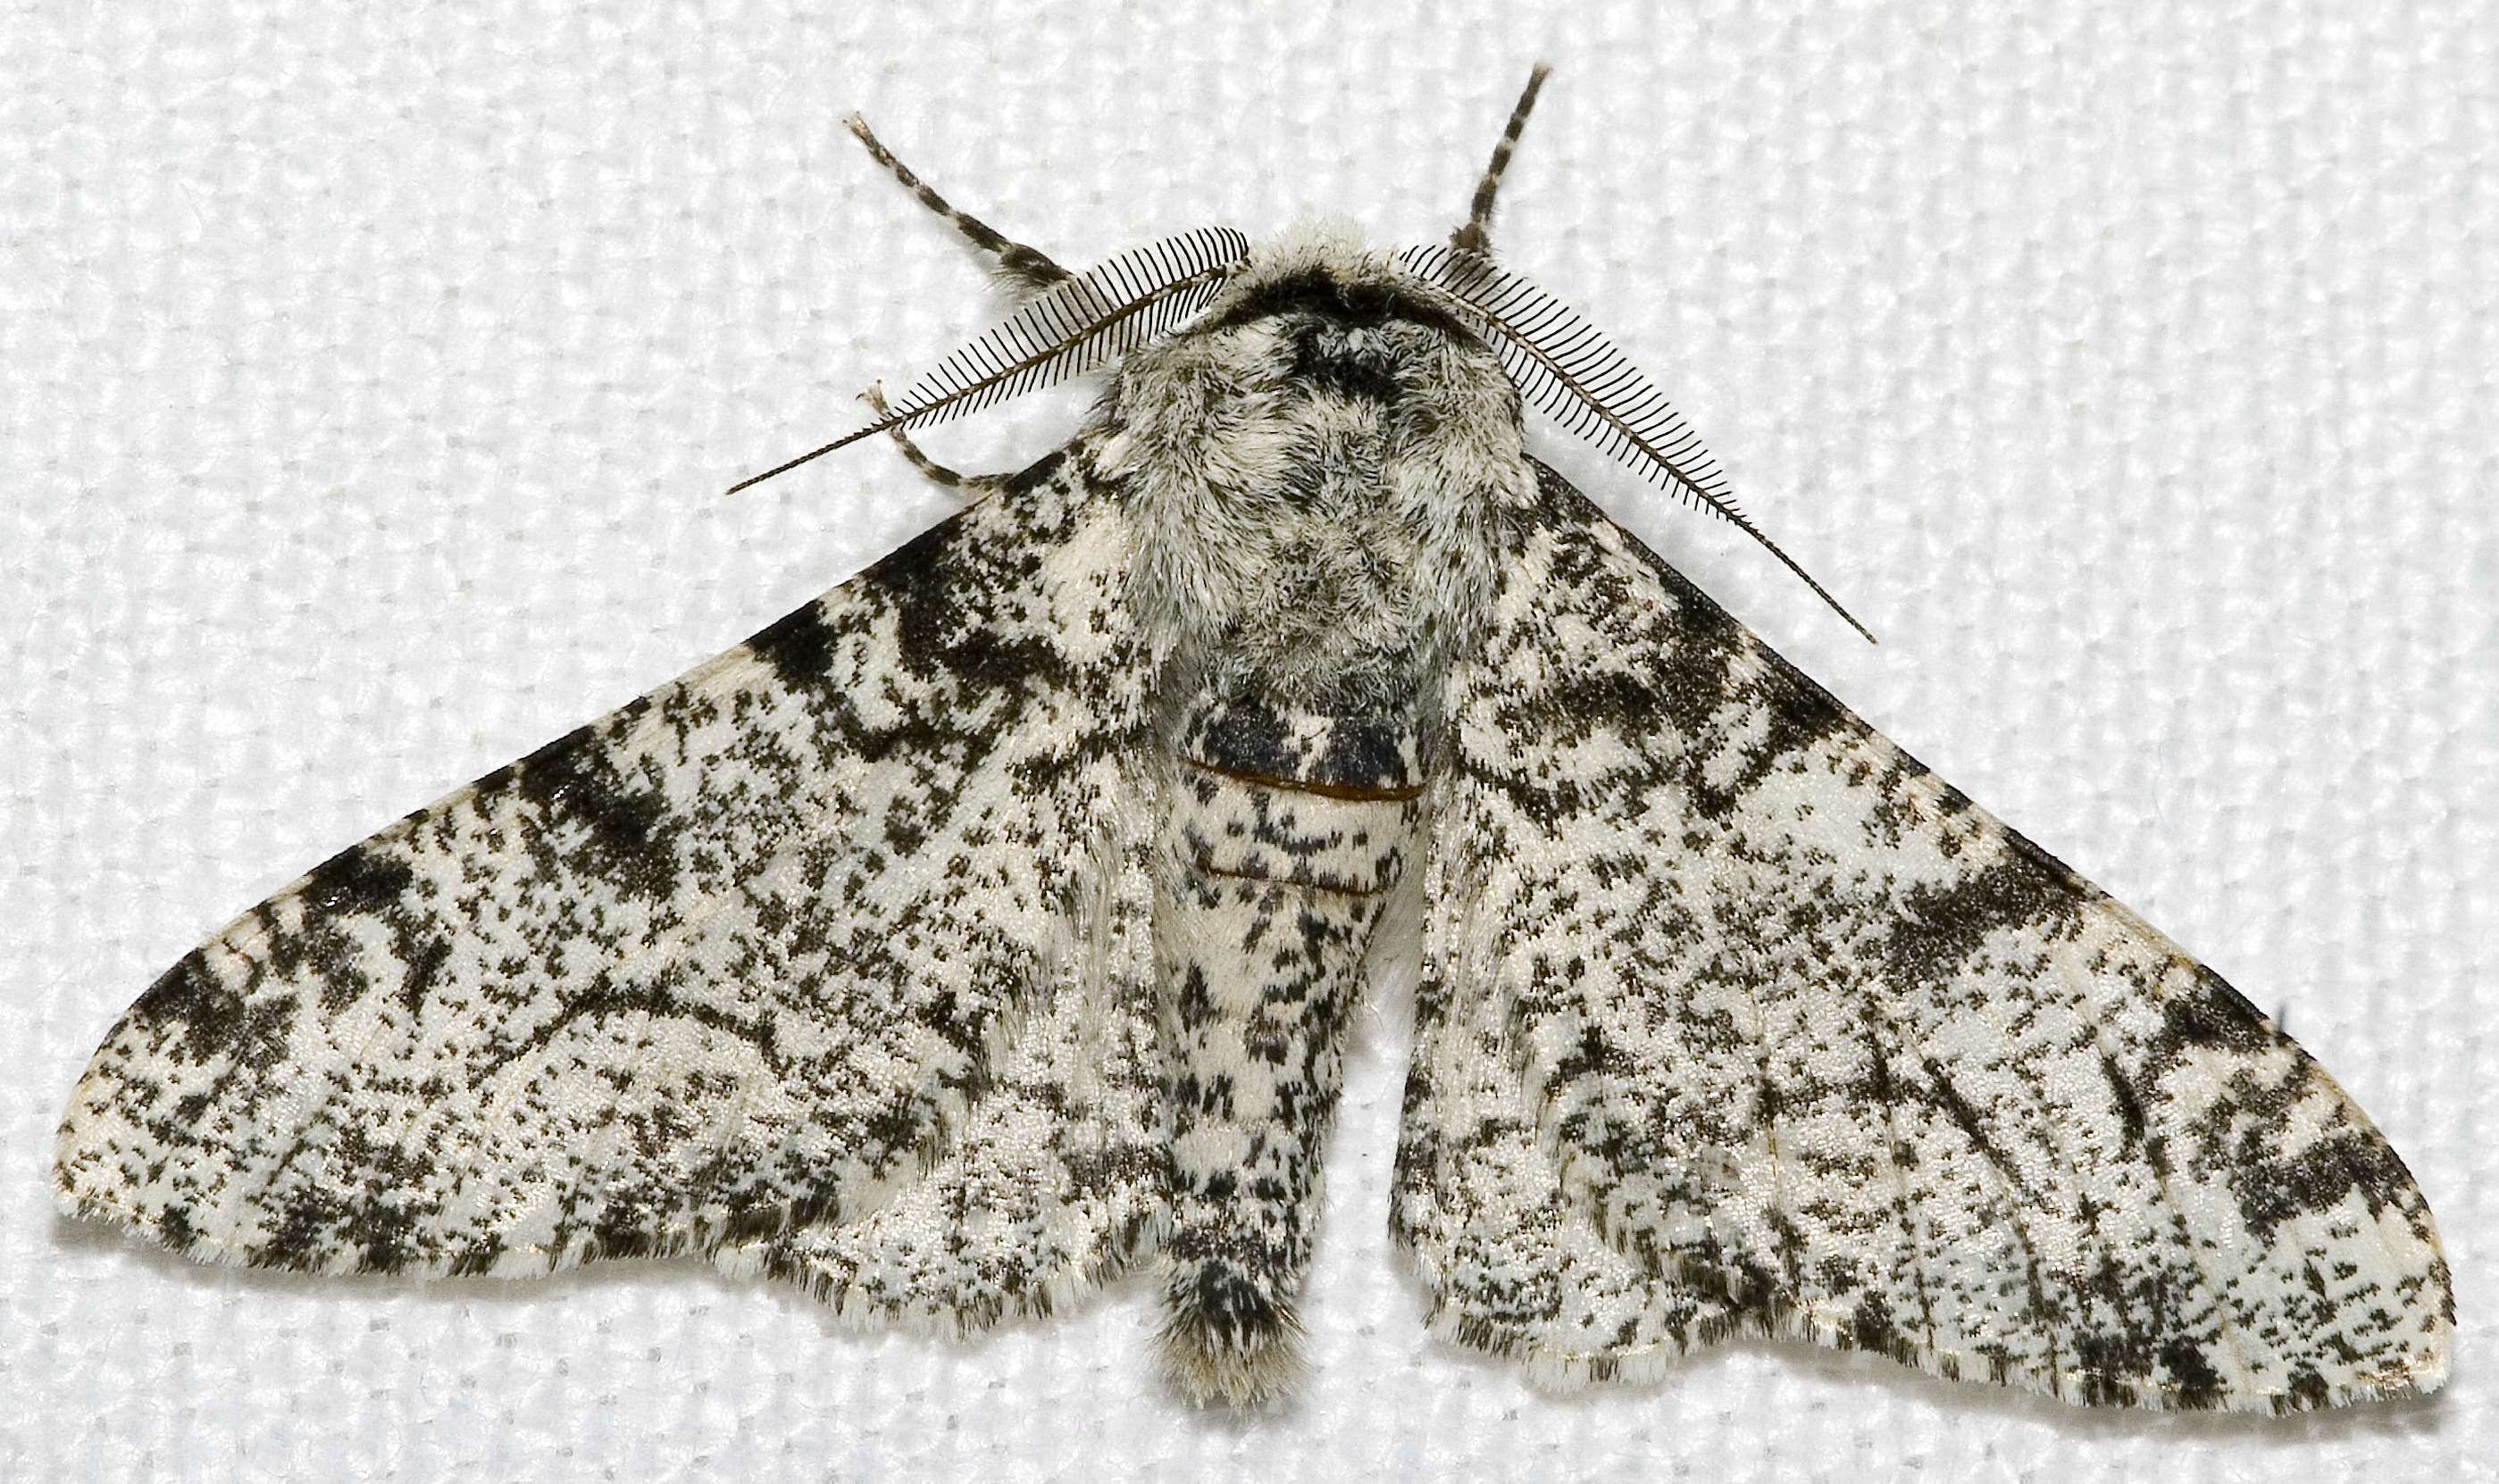
\includegraphics[width=0.7\linewidth]{./figures/evolution/Biston.betularia.7200} 

}

\caption{\href{https://commons.wikimedia.org/wiki/File:Biston.betularia.7200.jpg}{Biston betularia f.~typica, the white-bodied peppered moth.}}\label{fig:whitepeppered}
\end{figure}



\begin{figure}

{\centering 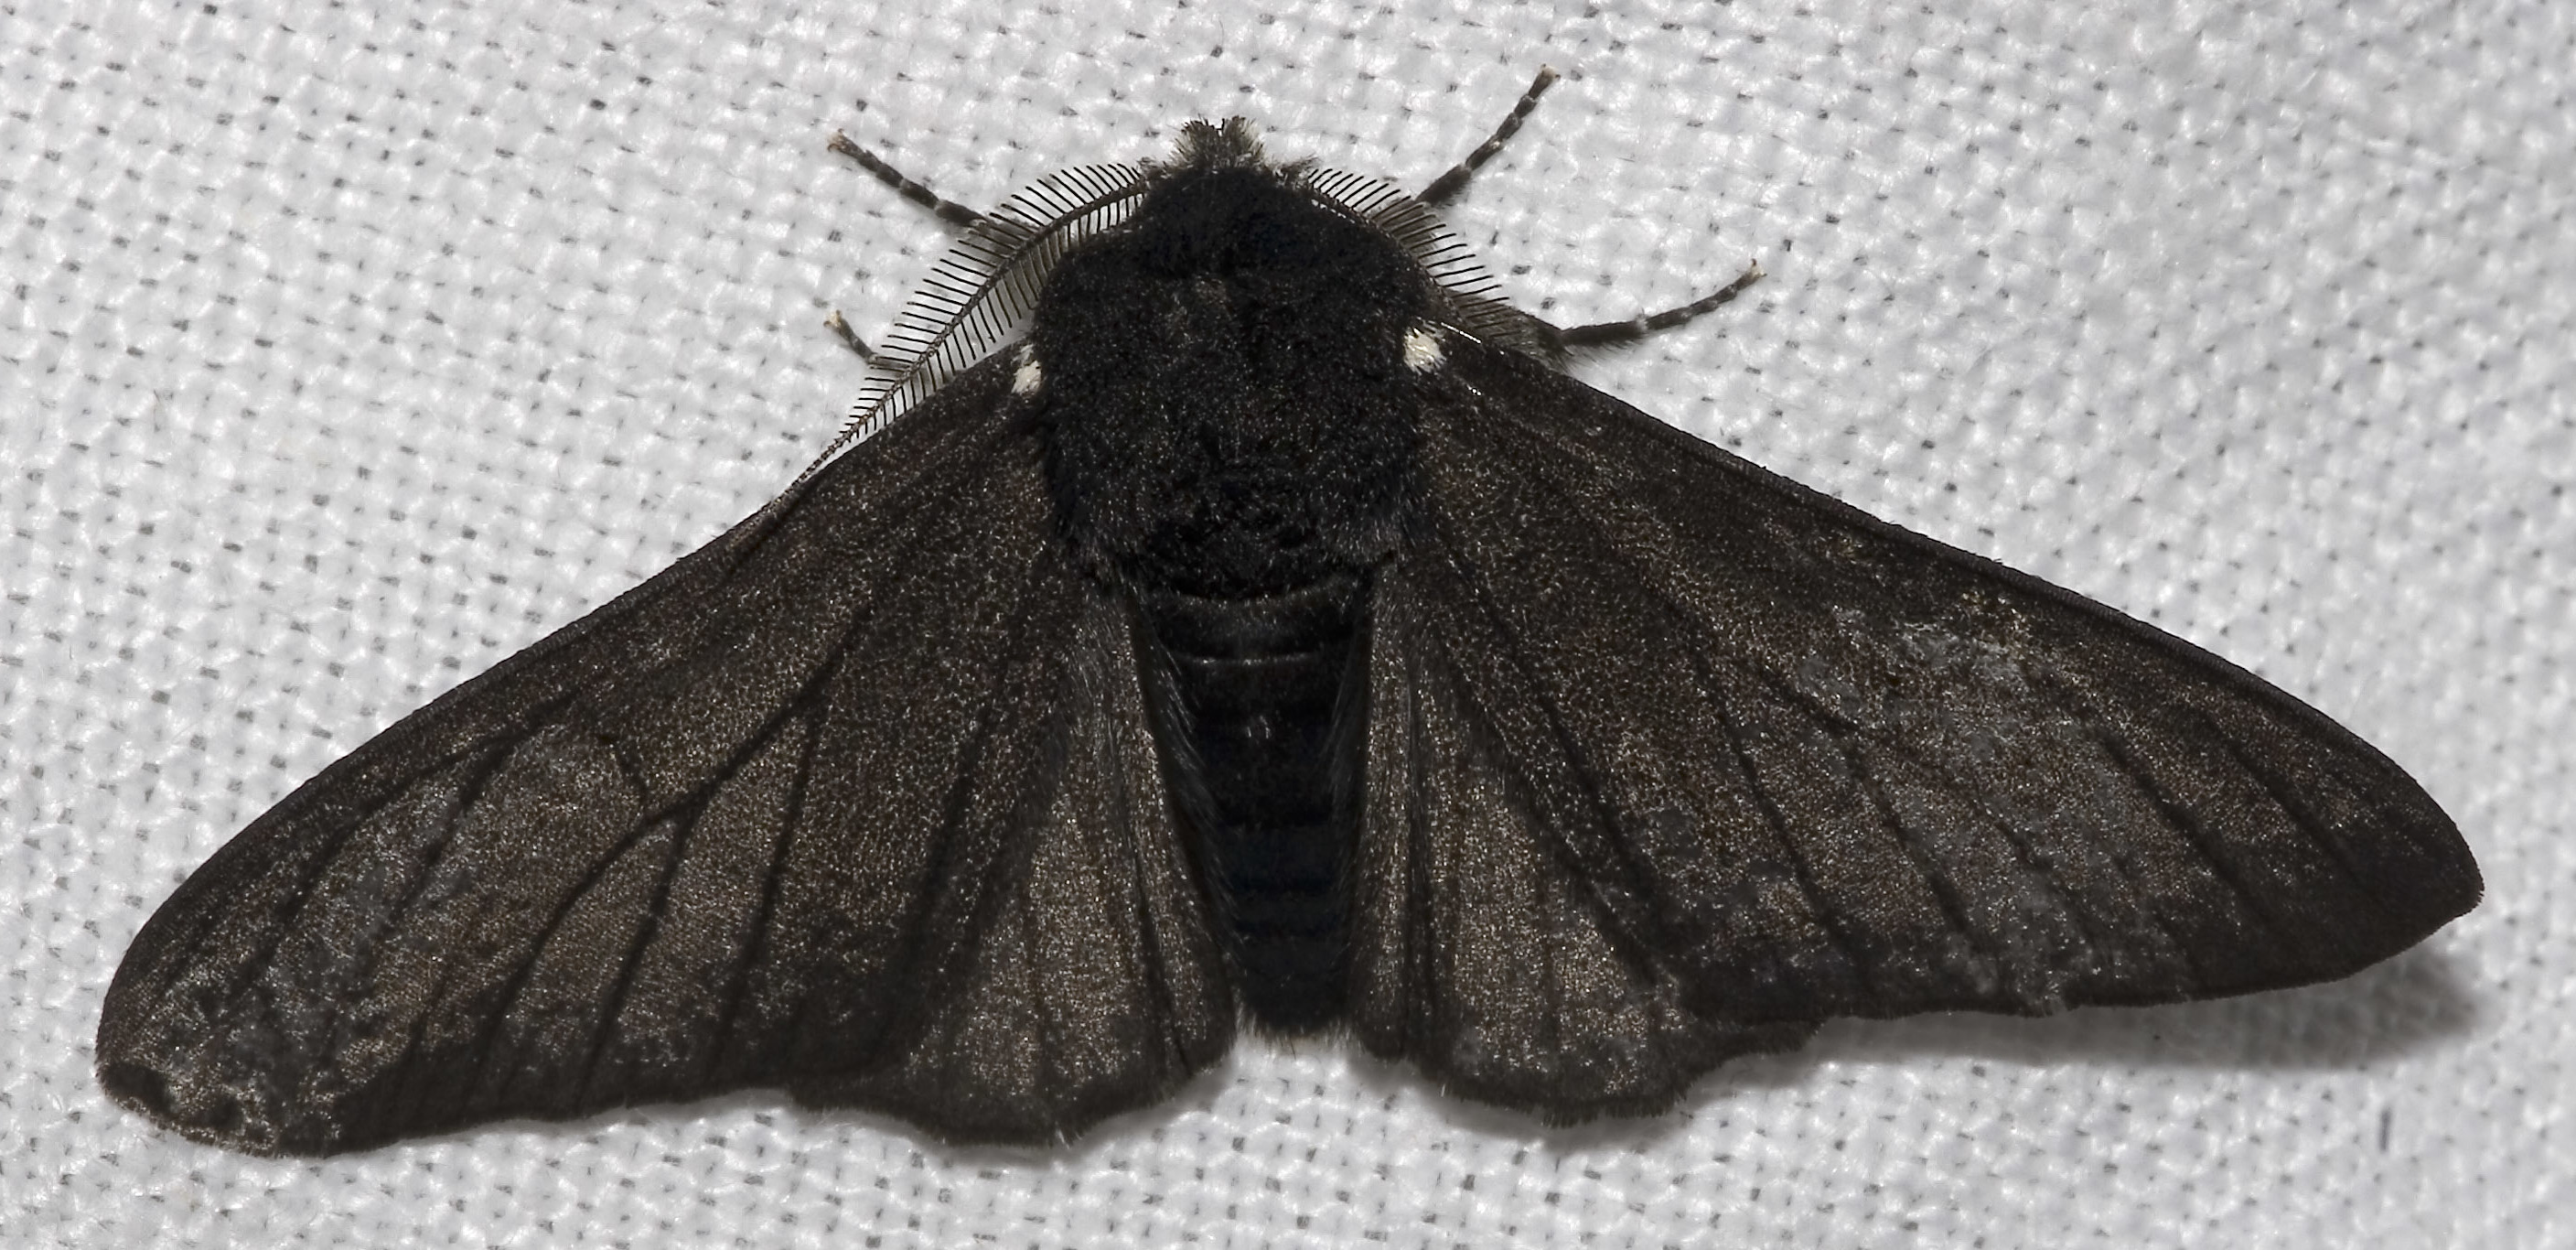
\includegraphics[width=0.7\linewidth]{./figures/evolution/Biston.betularia.f.carbonaria.7209} 

}

\caption{\href{https://commons.wikimedia.org/wiki/File:Biston.betularia.f.carbonaria.7209.jpg}{Biston betularia f.~carbonaria, the black-bodied peppered moth.}}\label{fig:carbonaramoth}
\end{figure}

The dark-coloured or melanic form of the peppered moth (var. carbonaria) was not known before 1811. After field collection in 1848 from Manchester, an industrial city in England, the frequency of the variety was found to have increased drastically. By the end of the 19th century it almost completely outnumbered the original light-coloured type (var. typica), with a record of 98\% in 1895. The evolutionary importance of the moth was only speculated upon during Darwin's lifetime. It was 14 years after Darwin's death, in 1896, that J.W. Tutt presented it as a case of natural selection. Due to this, the idea widely spread, and more people believed in Darwin's theory.

Bernard Kettlewell was the first to investigate the evolutionary mechanism behind peppered moth adaptation, between 1953 and 1956. He found that a light-coloured body was an effective camouflage in a clean environment, such as in Dorset, while the dark colour was beneficial in a polluted environment like in Birmingham. This selective survival was due to birds which easily caught dark moths on clean trees, and white moths on trees darkened with soot. The story, supported by Kettlewell's experiment, became the canonical example of Darwinian evolution and evidence for natural selection used in standard textbooks.



\begin{figure}

{\centering 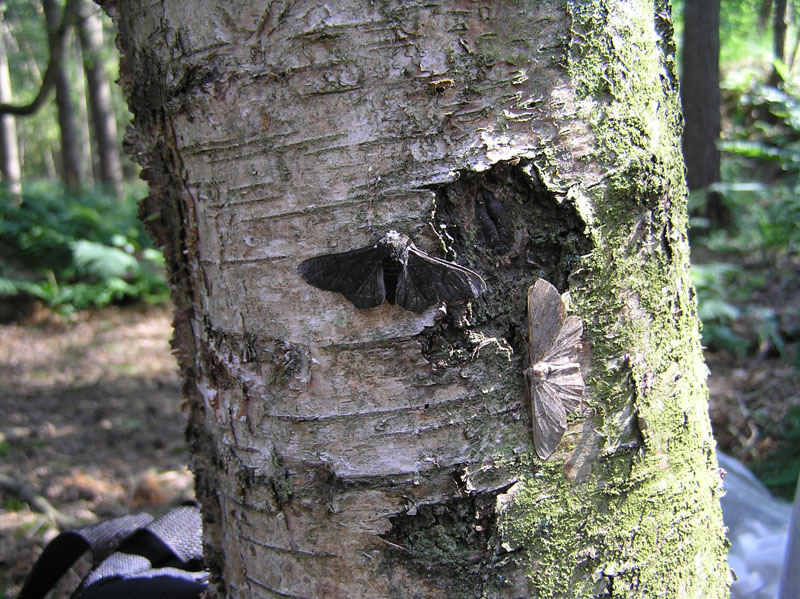
\includegraphics[width=0.7\linewidth]{./figures/evolution/Lichte_en_zwarte_versie_berkenspanner} 

}

\caption{\href{https://commons.wikimedia.org/wiki/File:Lichte_en_zwarte_versie_berkenspanner.jpg}{Typica and carbonaria morphs on the same tree.} The light-coloured typica (below the bark's scar) is nearly invisible on this pollution-free tree, camouflaging it from predators.}\label{fig:mothstree}
\end{figure}

However, failure to replicate the experiment and criticism of Kettlewell's methods by Theodore David Sargent in the late 1960s led to general skepticism. When Judith Hooper's Of Moths and Men was published in 2002, Kettlewell's story was more sternly attacked, accused of fraud, and became widely disregarded. The criticism became a major argument for creationists. Michael Majerus was the principal defender. His seven-year experiment beginning in 2001, the most elaborate of its kind in population biology, the results of which were published posthumously in 2012, vindicated Kettlewell's work in great detail. This restored peppered moth evolution as ``the most direct evidence'', and ``one of the clearest and most easily understood examples of Darwinian evolution in action''.

Before the Industrial Revolution, the black peppered moth was rare. The first black specimen (of unknown origin) was kept in the University of Oxford in 1811. The first live specimen was caught by R.S. Edleston in Manchester, England in 1848, but he reported this only 16 years later in 1864 in the journal Entomologist. Edleston notes that by 1864 it was the more common type of moth in his garden in Manchester. The light-bodied moths were able to blend in with the light-coloured lichens and tree bark, and the less common black moth was more likely to be eaten by birds. As a result of the common light-coloured lichens and English trees, therefore, the light-coloured moths were much more effective at hiding from predators, and the frequency of the dark allele was about 0.01\%.

During the early decades of the Industrial Revolution in England, the countryside between London and Manchester became blanketed with soot from the new coal-burning factories. Many of the light-bodied lichens died from sulphur dioxide emissions, and the trees became darkened. This led to an increase in bird predation for light-coloured moths, as they no longer blended in as well in their polluted ecosystem: indeed, their bodies now dramatically contrasted with the colour of the bark. Dark-coloured moths, on the other hand, were camouflaged very well by the blackened trees. The population of dark-coloured moth rapidly increased. By the mid-19th century, the number of dark-coloured moths had risen noticeably, and by 1895, the percentage of dark-coloured moths in Manchester was reported at 98\%, a dramatic change (of almost 100\%) from the original frequency. This effect of industrialization in body colour led to the coining of the term ``industrial melanism''.

The implication that industrial melanism could be evidence supporting Charles Darwin's theory of natural selection was noticed during his lifetime. Albert Brydges Farn (1841--1921), a British entomologist, wrote to Darwin on 18 November 1878 to discuss his observation of colour variations in the Annulet moth (then Gnophos obscurata, now Charissa obscurata). He noted the existence of dark moths in peat in the New Forest, brown moths on clay and red soil in Herefordshire, and white moths on chalk cliffs in Lewes, then suggested this variation was an example of ``survival of the fittest''. He told Darwin that he had found dark moths on a chalk slope where the foliage had been blackened by smoke from lime kilns, and he had also heard that white moths had become less common at Lewes after lime kilns had been in operation for a few years. Darwin does not seem to have responded to this information, possibly because he thought natural selection would be a much slower process. A scientific explanation of moth colouration was only published in 1896, 14 years after Darwin's death, when J.W. Tutt explicitly linked peppered moth melanism to natural selection.

\hypertarget{outcomes-of-evolution}{%
\section{Outcomes of Evolution}\label{outcomes-of-evolution}}

Evolution influences every aspect of the form and behaviour of organisms. Most prominent are the specific behavioural and physical adaptations that are the outcome of natural selection. These adaptations increase fitness by aiding activities such as finding food, avoiding predators or attracting mates. Organisms can also respond to selection by cooperating with each other, usually by aiding their relatives or engaging in mutually beneficial symbiosis. In the longer term, evolution produces new species through splitting ancestral populations of organisms into new groups that cannot or will not interbreed.

These outcomes of evolution are distinguished based on time scale as macroevolution versus microevolution. Macroevolution refers to evolution that occurs at or above the level of species, in particular speciation and extinction; whereas microevolution refers to smaller evolutionary changes within a species or population, in particular shifts in allele frequency and adaptation. In general, macroevolution is regarded as the outcome of long periods of microevolution. Thus, the distinction between micro- and macroevolution is not a fundamental one---the difference is simply the time involved. However, in macroevolution, the traits of the entire species may be important. For instance, a large amount of variation among individuals allows a species to rapidly adapt to new habitats, lessening the chance of it going extinct, while a wide geographic range increases the chance of speciation, by making it more likely that part of the population will become isolated. In this sense, microevolution and macroevolution might involve selection at different levels---with microevolution acting on genes and organisms, versus macroevolutionary processes such as species selection acting on entire species and affecting their rates of speciation and extinction.

A common misconception is that evolution has goals, long-term plans, or an innate tendency for ``progress'', as expressed in beliefs such as orthogenesis and evolutionism; realistically however, evolution has no long-term goal and does not necessarily produce greater complexity. Although complex species have evolved, they occur as a side effect of the overall number of organisms increasing and simple forms of life still remain more common in the biosphere. For example, the overwhelming majority of species are microscopic prokaryotes, which form about half the world's biomass despite their small size, and constitute the vast majority of Earth's biodiversity. Simple organisms have therefore been the dominant form of life on Earth throughout its history and continue to be the main form of life up to the present day, with complex life only appearing more diverse because it is more noticeable. Indeed, the evolution of microorganisms is particularly important to modern evolutionary research, since their rapid reproduction allows the study of experimental evolution and the observation of evolution and adaptation in real time.

\hypertarget{adaptation}{%
\subsection{Adaptation}\label{adaptation}}

Adaptation is the process that makes organisms better suited to their habitat. Also, the term adaptation may refer to a trait that is important for an organism's survival. For example, the adaptation of horses' teeth to the grinding of grass. By using the term adaptation for the evolutionary process and adaptive trait for the product (the bodily part or function), the two senses of the word may be distinguished. Adaptations are produced by natural selection. The following definitions are due to Theodosius Dobzhansky:

Adaptation is the evolutionary process whereby an organism becomes better able to live in its habitat or habitats.
Adaptedness is the state of being adapted: the degree to which an organism is able to live and reproduce in a given set of habitats.
An adaptive trait is an aspect of the developmental pattern of the organism which enables or enhances the probability of that organism surviving and reproducing.
Adaptation may cause either the gain of a new feature, or the loss of an ancestral feature. An example that shows both types of change is bacterial adaptation to antibiotic selection, with genetic changes causing antibiotic resistance by both modifying the target of the drug, or increasing the activity of transporters that pump the drug out of the cell. Other striking examples are the bacteria Escherichia coli evolving the ability to use citric acid as a nutrient in a long-term laboratory experiment, Flavobacterium evolving a novel enzyme that allows these bacteria to grow on the by-products of nylon manufacturing, and the soil bacterium Sphingobium evolving an entirely new metabolic pathway that degrades the synthetic pesticide pentachlorophenol. An interesting but still controversial idea is that some adaptations might increase the ability of organisms to generate genetic diversity and adapt by natural selection (increasing organisms' evolvability).

Adaptation occurs through the gradual modification of existing structures. Consequently, structures with similar internal organisation may have different functions in related organisms. This is the result of a single ancestral structure being adapted to function in different ways. The bones within bat wings, for example, are very similar to those in mice feet and primate hands, due to the descent of all these structures from a common mammalian ancestor. However, since all living organisms are related to some extent, even organs that appear to have little or no structural similarity, such as arthropod, squid and vertebrate eyes, or the limbs and wings of arthropods and vertebrates, can depend on a common set of homologous genes that control their assembly and function; this is called deep homology.



\begin{figure}

{\centering 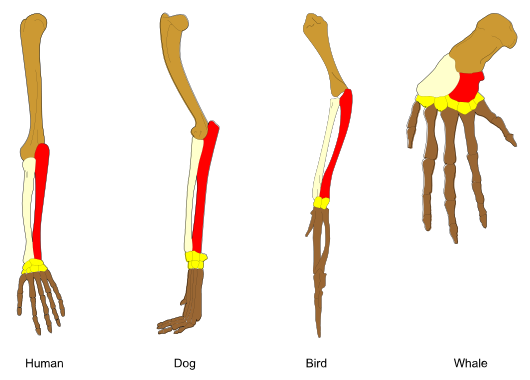
\includegraphics[width=0.7\linewidth]{./figures/evolution/Homology_vertebrates-en} 

}

\caption{\href{https://commons.wikimedia.org/wiki/File:Homology_vertebrates-en.svg}{Homologous bones in the limbs of tetrapods. The bones of these animals have the same basic structure, but have been adapted for specific uses.}}\label{fig:homologousbones}
\end{figure}

During evolution, some structures may lose their original function and become vestigial structures. Such structures may have little or no function in a current species, yet have a clear function in ancestral species, or other closely related species. Examples include pseudogenes, the non-functional remains of eyes in blind cave-dwelling fish, wings in flightless birds, the presence of hip bones in whales and snakes, and sexual traits in organisms that reproduce via asexual reproduction. Examples of vestigial structures in humans include wisdom teeth, the coccyx, the vermiform appendix, and other behavioural vestiges such as goose bumps and primitive reflexes.

However, many traits that appear to be simple adaptations are in fact exaptations: structures originally adapted for one function, but which coincidentally became somewhat useful for some other function in the process. One example is the African lizard Holaspis guentheri, which developed an extremely flat head for hiding in crevices, as can be seen by looking at its near relatives. However, in this species, the head has become so flattened that it assists in gliding from tree to tree---an exaptation. Within cells, molecular machines such as the bacterial flagella and protein sorting machinery evolved by the recruitment of several pre-existing proteins that previously had different functions. Another example is the recruitment of enzymes from glycolysis and xenobiotic metabolism to serve as structural proteins called crystallins within the lenses of organisms' eyes.

An area of current investigation in evolutionary developmental biology is the developmental basis of adaptations and exaptations. This research addresses the origin and evolution of embryonic development and how modifications of development and developmental processes produce novel features. These studies have shown that evolution can alter development to produce new structures, such as embryonic bone structures that develop into the jaw in other animals instead forming part of the middle ear in mammals. It is also possible for structures that have been lost in evolution to reappear due to changes in developmental genes, such as a mutation in chickens causing embryos to grow teeth similar to those of crocodiles. It is now becoming clear that most alterations in the form of organisms are due to changes in a small set of conserved genes.

\hypertarget{coevolution}{%
\subsection{Coevolution}\label{coevolution}}

Interactions between organisms can produce both conflict and cooperation. When the interaction is between pairs of species, such as a pathogen and a host, or a predator and its prey, these species can develop matched sets of adaptations. Here, the evolution of one species causes adaptations in a second species. These changes in the second species then, in turn, cause new adaptations in the first species. This cycle of selection and response is called coevolution. An example is the production of tetrodotoxin in the rough-skinned newt and the evolution of tetrodotoxin resistance in its predator, the common garter snake. In this predator-prey pair, an evolutionary arms race has produced high levels of toxin in the newt and correspondingly high levels of toxin resistance in the snake.


